We compare the performances of the proposed schemes with the system having \me{K = 20} and \me{N_\mrm{T} = 4}. ZF based precoder design is employed at the transmitter to provide interference free transmission to the multiplexed users. The path loss is assumed to be equal among the users in order to provide a fair comparison between the scheduling schemes with sum rate maximizing objective.
\begin{figure}
\centering
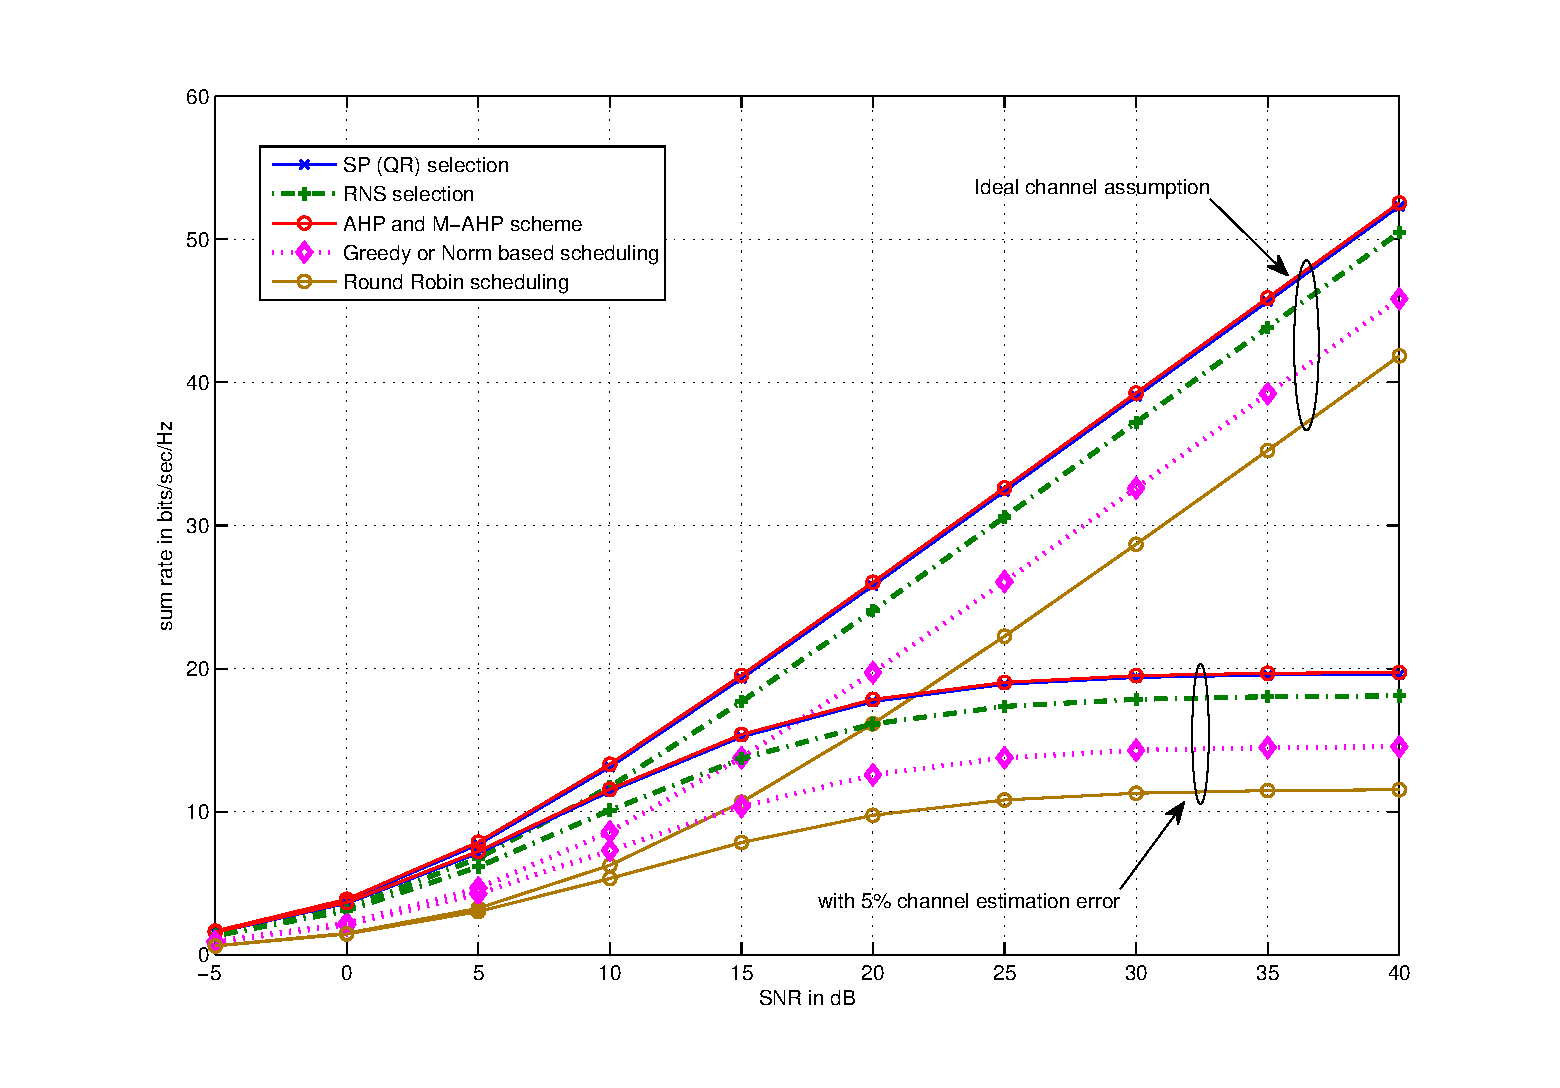
\includegraphics[width=1.0\columnwidth]{single-bs-7}
\vspace{-0.2in}
\caption[short]{Sum rate for \me{\card{\mc{U}} = 20, \, N_\mrm{T} = 4, \, N_\mrm{R} = 1}}
\vspace{-0.1in}
\label{single-bs-f1}
\end{figure}

Fig. \ref{single-bs-f1} compares the sum rate plot attained by scheduling schemes discussed so far. The \ac{AHP} scheme, which selects the user by considering not only the existing set of users \me{\mc{S}} but also the other users in the set \me{\mc{U} \bs \mc{S}}, performs noticeably better than the SP based scheme.  The gain achieved is not significant when compared with the complexity involved in the selection procedure. Fig. \ref{single-bs-f1} also shows the performance of the \ac{RNS} based selection scheme, which performs marginally close to the SP scheme with a significant reduction in the complexity. The \ac{RR} and norm based scheduling are also compared for illustrative purposes along with the \ac{SP} scheme. The figure also shows the gain degradation in the presence of estimation error in the channel. Adding estimation error of \me{5\%}, degrades the sum rate noticeably. For example, at \me{25} dB SNR, the loss is almost \me{10} bits with the estimation error. The performance loss is mainly attributed to the interference leakage by the \ac{ZF} precoder when the channel used is imperfect at the transmitter.
\begin{figure}
\centering
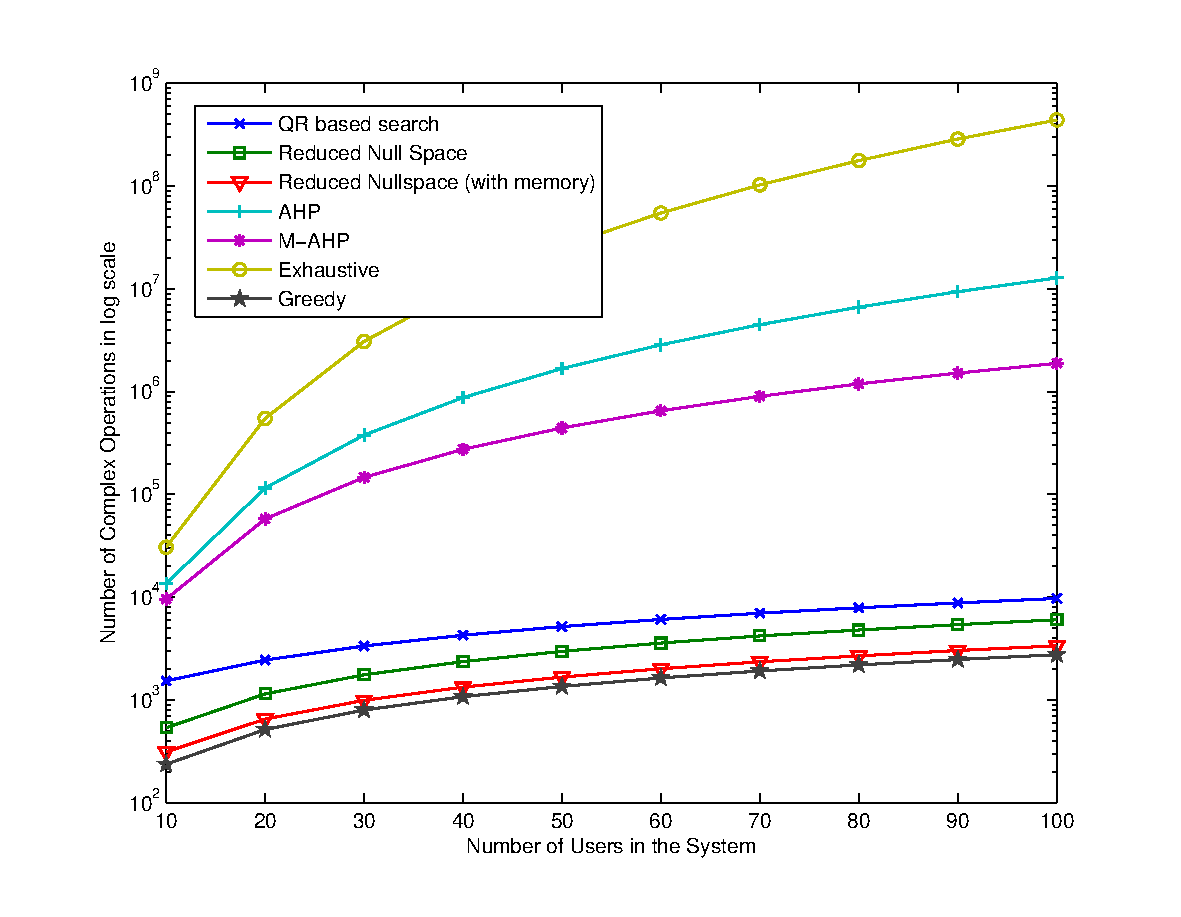
\includegraphics[width=1.0\columnwidth]{single-bs-6}
\vspace{-0.2in}
\caption[short]{Scaling of complexity over users for \me{N_\mrm{T} = 4, \, N_\mrm{R} = 1} system}
\vspace{-0.1in}
\label{single-bs-f2}
\end{figure}

Fig. \ref{single-bs-f2} compares the complexity involved in the metric calculation for different scheduling schemes with the number of users being the variable. The complexity involved with the \ac{AHP} based selection scheme is of polynomial order due to \me{K \frac{(K + 1)}{2}} pairs involved in the computation. The \ac{RNS} selection performs marginally inferior to the SP scheme, which requires more complex computations for the metric calculation as shown in Fig. \ref{single-bs-f2}. The \ac{RNS} scheme can be reduced further when the memory is utilized to save the earlier projections over the normalized channels in the set \me{\mc{S}}.

Fig. \ref{single-bs-f3} compares the sum rate performance of the above discussed scheduling schemes with different numbers of users. It is evident that the \ac{AHP} and \ac{M-AHP} schemes perform better over other schemes. The performance of \ac{RNS} performs close with the SP based selection with reduced complexity involved in evaluating the metric for the selection. As the number of users increases, the complexity of all scheduling schemes increases linearly except that of the \ac{AHP} scheme, which is of polynomial order. As the number of users in the system increases, the rate loss between the \ac{SP} scheme and the \ac{RNS} scheme reduces as shown in Fig. \ref{single-bs-f3}. The \ac{RNS} scheme provides two-fold benefits by reducing the load on the processor and also performs closer to the other near-optimal schemes.
\begin{figure}
\centering
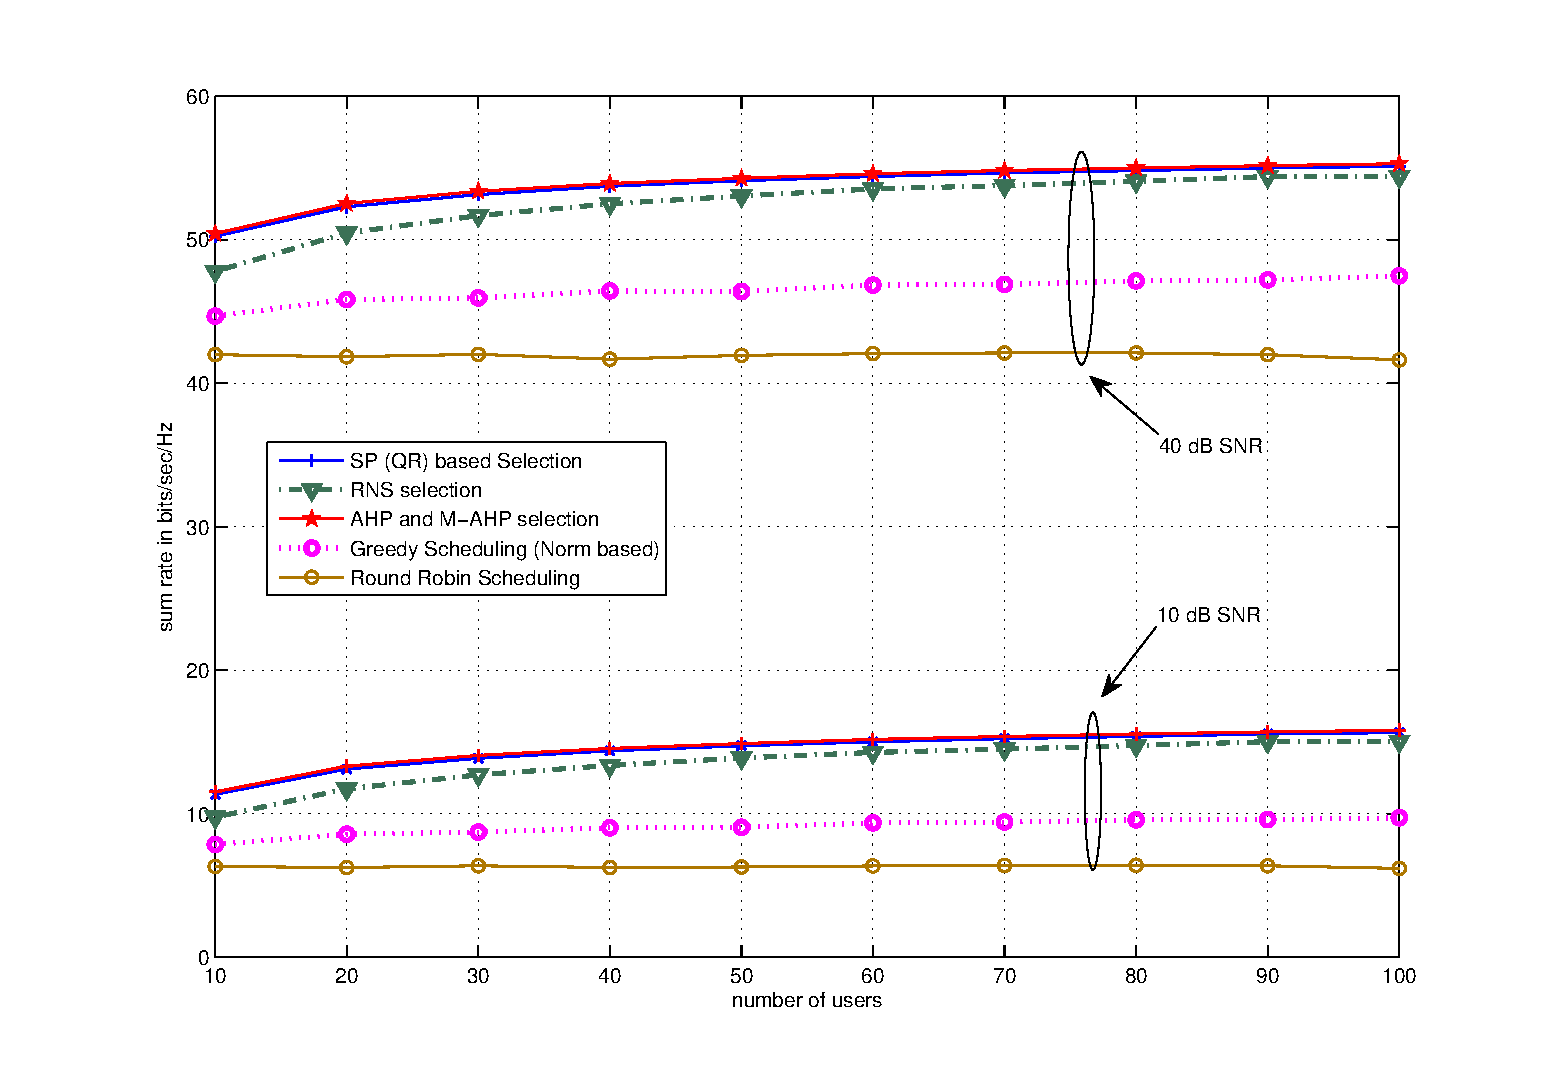
\includegraphics[width=1.0\columnwidth]{single-bs-5}
\vspace{-0.2in}
\caption[short]{Sum rate with \me{N_\mrm{T} = 4, \, N_\mrm{R} = 1} with variable users}
\vspace{-0.1in}
\label{single-bs-f3}
\end{figure}
